\documentclass{../../oss-apphys-exam}
\usepackage{bm}
\usepackage{circuitikz} % to draw circuits!

\begin{document}
\genheader

\gentitle{C}{MAGNETISM, PART 1}

\genmultidirections
\raggedcolumns
\begin{multicols*}{2}
  \begin{questions}
    \question An electron is moving downward toward the bottom of the page when
    it passes through a region of magnetic field, as shown in the figure by
    the shaded area. The electron travels along a path that takes it through
    the spot marked $X$. The gravitational force on the electron is very
    small. What is the direction of the magnetic field?
    \begin{center}
      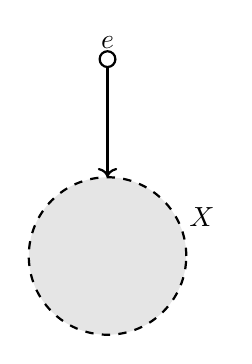
\begin{tikzpicture}
        \draw[thick,dashed,fill=gray!20](0,0) circle(1);
        \node at (1.2,.5) {$X$};
        \draw[thick](0,2.5) circle(.1) node[above]{$e$};
        \draw[thick,->](0,2.4)--(0,1);
      \end{tikzpicture}
    \end{center}
    \begin{choices}
      \choice Toward the bottom of the page
      \choice Toward the top of the page
      \choice Out of the page
      \choice Into the page
    \end{choices}
    
    \question Two long parallel wires carry currents ($I_A$ and $I_B$), as shown
    in the figure. Current $I_A$ in the left wire is twice that of current
    $I_B$ in the right wire. The magnetic force on the right wire is $F$. What
    is the magnetic force on the left wire in terms of $F$?
    \begin{center}
      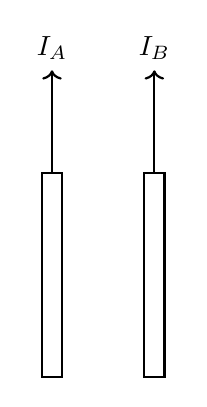
\begin{tikzpicture}[scale=1.3]
        \begin{scope}[thick]
          \draw(0,0) rectangle(.2,2);
          \draw(1,0) rectangle(1.2,2);
          \draw[->](.1,2)--(.1,3) node[above]{$I_A$};
          \draw[->](1.1,2)--(1.1,3) node[above]{$I_B$};
        \end{scope}
      \end{tikzpicture}
    \end{center}
    \begin{choices}
      \choice $F$ in the same direction
      \choice $F$ in the opposite direction
      \choice $F/2$ in the same direction
      \choice $F/2$ in the opposite direction
    \end{choices}
    \vspace{.7in}
    
%  \item An iron magnet is broken in half at the midpoint between its north
%    andsouth ends. What is the result?
%    \begin{choices}
%      \choice A separate north pole and south pole, each with the same
%      magnetic strength as the original magnet
%      \choice A separate north pole and south pole, each with half the magnetic
%      strength of the original magnet 
%      \choice Two separate north-south magnets, each with the same magnetic
%      strength as the original magnet
%      \choice Two separate north-south magnets, each with half the magnetic
%      strength of the original magnet
%    \end{choices}
%    \vspace{.7in}

  \item The figure below shows the microscopic dipoles inside two metal objects.
    Copper is diamagnetic. Iron is ferromagnetic. Which of the following
    best depicts the microscopic internal dipole position when the objects
    are placed in a strong, external magnetic field directed toward the top
    of the page?
    \begin{center}
      \pic{.13}{copper-iron}

      \pic{.45}{domains}
    \end{center}
    
    \question A magnetic field, directed into the page, is placed between two
    charged capacitor plates, as shown in the figure. The magnetic and electric
    fields are adjusted so a proton moving at a velocity of $\varv$ will pass
    straight through the fields. The speed of the proton is doubled to $2\varv$.
    Which of the following force diagrams most accurately depicts the forces
    acting on the proton when traveling at $2\varv$?
    \begin{center}
      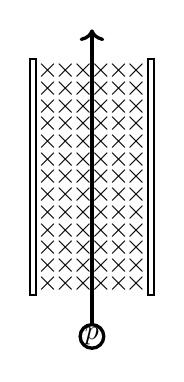
\begin{tikzpicture}[scale=.75]
        \begin{scope}[thick]
          \draw(0,0) rectangle(.1,4);
          \draw(2,0) rectangle(2.1,4);
          \foreach\x in {.3,.6,...,2}{
            \foreach\y in {.2,.5,...,4} \node at (\x,\y) {$\times$};
          }
          \draw[very thick,->](1.05,-.5)--(1.05,4.5);
          \draw[very thick](1.05,-.7) circle(.2) node{$p$};
        \end{scope}
      \end{tikzpicture}
    \end{center}
    \begin{choices}
      \choice
      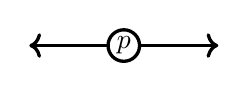
\begin{tikzpicture}
        \draw[very thick](0,0) circle(.2) node{$p$};
        \draw[very thick,->](.2,0)--(1.2,0);
        \draw[very thick,->](-.2,0)--(-1.2,0);
      \end{tikzpicture}
      
      \choice
      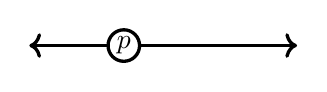
\begin{tikzpicture}
        \draw[very thick](0,0) circle(.2) node{$p$};
        \draw[very thick,->](.2,0)--(2.2,0);
        \draw[very thick,->](-.2,0)--(-1.2,0);
      \end{tikzpicture}

      \choice
      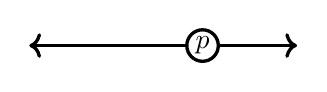
\begin{tikzpicture}
        \draw[very thick](0,0) circle(.2) node{$p$};
        \draw[very thick,->](.2,0)--(1.2,0);
        \draw[very thick,->](-.2,0)--(-2.2,0);
      \end{tikzpicture}
      
      \choice
      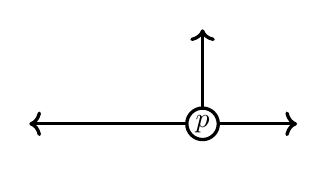
\begin{tikzpicture}
        \draw[very thick](0,0) circle(.2) node{$p$};
        \draw[very thick,->](.2,0)--(1.2,0);
        \draw[very thick,->](-.2,0)--(-2.2,0);
        \draw[very thick,->](0,.2)--(0,1.2);
      \end{tikzpicture}
    \end{choices}
    
    \question Which of the following is true concerning the force on the
    current-carrying wire due to the electron?
    \begin{center}
      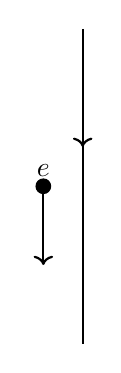
\begin{tikzpicture}
        \draw[thick,->](0,4)--(0,2.5);
        \draw[thick](0,3)--(0,0);
        \fill(-.5,2) circle(.1) node[above] {$e$};
        \draw[thick,->](-.5,2)--(-.5,1) node[below]{$\varv$};
      \end{tikzpicture}
    \end{center}
    \begin{choices}
      \choice The force is directed toward the right.
      \choice The force is directed toward the left.
      \choice The force is directed into the page.
      \choice There is no force on the current-carrying wire due to the
      electron.
    \end{choices}

    \question A loop of wire in the plane of the page carries a clockwise
    current $I$ and is placed in a magnetic field that is directed into the
    page as shown. Which of the following will happen as a result of the wire
    loop being in the magnetic field?
    \begin{center}
      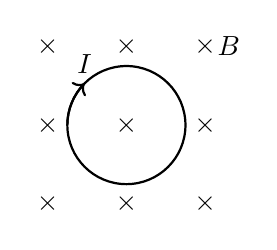
\begin{tikzpicture}
        \foreach \x in {-1,0,1}{
          \foreach \y in {-1,0,1}{
            \node at (\x,\y) {$\times$};
          }
        }
        \draw[thick](0,0) circle(.75);
        \draw[thick,->](-.75,0) arc(180:135:.75) node[above]{$I$};
        \node at (1.3,1) {$B$};
      \end{tikzpicture}
    \end{center}
    \begin{choices}
      \choice The wire loop will rotate clockwise.
      \choice The wire loop will rotate counterclockwise.
      \choice The wire loop will flip on a horizontal axis through its center.
      \choice The wire loop will expand in size.
      \choice The wire loop will contract in size.
    \end{choices}
    \columnbreak
    
    \uplevel{
      \textbf{Questions \ref{q:2wires1}--\ref{q:2wires2}}
  
      Two wires carry currents $2A$ and $4A$ in the directions shown. Point $P$
      is a distance $r$ from the wire carrying $2A$, and a distance $2r$ from
      the wire carrying $4A$.
      \begin{center}
        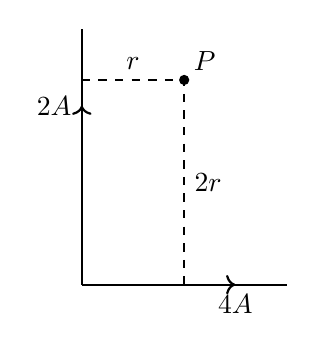
\begin{tikzpicture}[scale=1.3]
          \draw[thick](0,0)--(2,0);
          \draw[thick,->](0,0)--(1.5,0) node[below]{$4A$};
          \draw[thick](0,0)--(0,2.5);
          \draw[thick,->](0,0)--(0,1.75) node[left]{$2A$};
          \draw[thick,dashed](0,2)--(1,2)node[midway,above]{$r$}
          --(1,0) node[midway,right]{$2r$};
          \fill[black](1,2) circle(.05) node[above right]{$P$};
        \end{tikzpicture}
      \end{center}
    }

    \question Which of the following statements is true?
    \begin{choices}
      \choice The magnetic field produced at point $P$ by the wire carrying
      $2A$ is greater than the magnetic field produced at point $P$ by the wire
      carrying $4A$, but opposite in direction.
      \choice The magnetic field produced at point $P$ by the wire carrying
      $2A$ is less than the magnetic field produced at point $P$ by the wire
      carrying $4A$, and in the same direction.
      \choice The magnetic field produced at point $P$ by the wire carrying
      $2A$ is equal to the magnetic field produced at point $P$ by the wire
      carrying $4A$, but opposite in direction.
      \choice The magnetic field produced at point $P$ by the wire carrying
      $2A$ is equal to the magnetic field produced at point $P$ by the wire
      carrying $4A$, and in the same direction.
      \choice The magnetic field produced at point $P$ by the wire carrying
      $2A$ is greater than the magnetic field produced at point $P$ by the wire
      carrying $4A$, and in the same direction.
    \end{choices}
    \label{q:2wires1}

    \question The magnitude of the resultant magnetic field at point $P$ due to
    the current in the two wires is
    \begin{choices}
      \choice zero
      \choice $\dfrac{\mu_0(2A)}{2\pi r}$
      \choice $\dfrac{\mu_0(2A)}{\pi r}$
      \choice $\dfrac{\mu_0(4A)}{2\pi r}$
      \choice $\dfrac{\mu_0(6A)}{4\pi r}$
    \end{choices}
    \label{q:2wires2}
    \columnbreak

    \question A dynamic microphone contains a magnet and a coil of wire
    connected to a movable diaphragm, as shown in the figure. Sound waves
    directed at the diaphragm generate a current in the wires leading from the
    coil. Which of the following helps to explain why this occurs?
    \cpic{.38}{mic}
    \begin{choices}
      \choice The area of the coil changes.
      \choice The magnitude of the magnetic field produced by the magnet
      changes.
      \choice The angle between the plane of the coil and the magnetic field
      produced by the magnet change.
      \choice The strength of the magnetic field in the plane of the coil
      changes.
    \end{choices}
    \vspace{.7in}
    \columnbreak

    \uplevel{
      \textbf{Questions \ref{q:2curr1}--\ref{q:2curr2}}

      Two wires are parallel to each other, one carrying twice the current as
      the other. The two currents flow in the same direction.
    }

    \question Which of the following is true of the forces the wires exert on
    each other?
    \begin{choices}
      \choice The wire with the larger current exerts a greater force on the
      other wire.
      \choice The wire with the smaller current exerts a greater force on the
      other wire.
      \choice The wires exert equal and opposite forces on each other.
      \choice The wires exert equal forces on each other, but in the same
      direction.
      \choice The net force between the wires is zero.
    \end{choices}
    \label{q:2curr1}
    \vspace{.7in}
    
    \question The direction of the force between the wires is
    \begin{choices}
      \choice repulsive
      \choice attractive
      \choice zero
      \choice into the page
      \choice out of the page
    \end{choices}
    \label{q:2curr2}
    \vspace{.7in}
    
    \uplevel{
      \textbf{Questions \ref{q:circ1}--\ref{q:circ2}}
      A negatively charged particle of mass $m$ and charge $q$ in a uniform
      magnetic field $B$ travels in a circular path of radius $r$.
      \begin{center}
        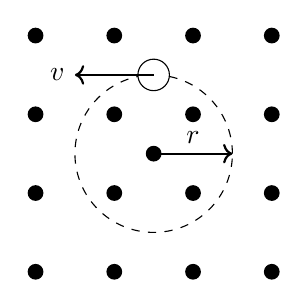
\begin{tikzpicture}
          \foreach \x in {0,...,3}{
            \foreach \y in {0,...,3}{
              \fill[black](\x,\y)circle(.1);
            }
          }
          \fill[black](1.5,1.5)circle(.1);
          \draw[thick,->](1.5,1.5)--(2.5,1.5) node[midway,above]{$r$};
          \draw[dashed](1.5,1.5) circle(1);
          \draw[fill=white](1.5,2.5) circle(.2);
          \draw[thick,->](1.5,2.5)--(.5,2.5) node[left]{$v$};
        \end{tikzpicture}
      \end{center}
    }

    \question In terms of the other given quantities, the charge-to-mass ratio
    $q/m$ of the particle is
    \begin{choices}
      \choice $\dfrac{Bv}r$
      \choice $\dfrac r{Bv}$
      \choice $\dfrac{rv}B$
      \choice $rvB$
      \choice $\dfrac v{rB}$
    \end{choices}
    \label{q:circ1}
    
    \question The work done by the magnetic field after two full revolutions of
    the charge is
    \begin{choices}
      \choice zero
      \choice $-qvB/rm$
      \choice $qvm/Br$
      \choice $-mBr/qv$
      \choice $-mqvBr$
    \end{choices}
    \label{q:circ2}
    
    \question A current is passed through an analog ammeter and the needle moves
    to indicate the current flowing through the circuit. Which of the
    following best explains how an analog ammeter works?
    \begin{choices}
      \choice Current is passed through the needle placed in a magnetic field,
      and the needle is attracted to the high side of the scale.
      \choice The needle is a magnet, and is attracted to a magnet on the high
      side of the scale.
      \choice The needle gathers an electrostatic charge from the current, and
      is attracted to an electrostatic charge on the high side of the scale.
      \choice Current is passed through a spring coil of wire placed in a
      magnetic field, and the coil rotates, moving the needle
      proportionally to the current in the coil.
      \choice Current flows through the needle, making it heavier, and it falls
      to the high side of the scale.
    \end{choices}
    \vspace{.7in}
    
%    \question An electric motor consists of a current-carrying loop of wire
%    mounted to an axle and turned at a slight angle in a magnetic field as
%    shown. The wire loop will
%    \cpic{.35}{motor-drawing}
%    \begin{choices}
%      \choice experience a torque and turn clockwise
%      \choice experience a torque and turn counterclockwise
%      \choice accelerate upward out of the magnetic field
%      \choice accelerate downward out of the magnetic field
%      \choice not experience a force or torque
%    \end{choices}
  \end{questions}
\end{multicols*}
\newpage

\genfreetitle{C}{MAGNETISM}{8}

\genfreedirections

% TAKEN FROM 2001 AP PHYSICS C EXAM FREE-RESPONSE QUESTION E&M 3
\begin{center}
  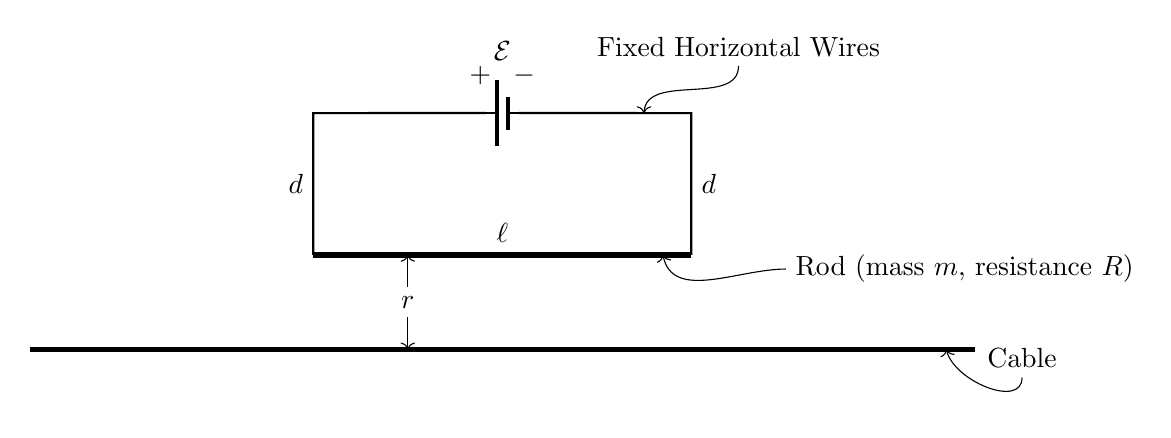
\begin{tikzpicture}[american voltages,scale=1.2]
    \draw[ultra thick](-5,0)--(5,0);
    \draw[line width=.8mm](-2,1)--(2,1) node[midway,above]{$\ell$};
    \draw[thick](-2,1)--(-2,2.5)node[midway,left]{$d$}
    to[battery1=$\mathcal E$](2,2.5)--(2,1) node[midway,right]{$d$};
    \draw[<->](-1,1)--(-1,0) node[midway,fill=white]{$r$};
    \draw[<-](4.7,0) to[in=270,out=-80](5.5,-.3) node[above]{Cable};
    \draw[<-](1.7,1) to[in=180,out=-80](3,.85)
    node[right]{Rod (mass $m$, resistance $R$)};
    \draw[<-](1.5,2.5) to[in=270,out=90](2.5,3)
    node[above]{Fixed Horizontal Wires};
  \end{tikzpicture}
\end{center}

\begin{questions}
  \question The circuit shown above consists of a battery of emf $\mathcal E$
  in series with a rod of length $\ell$, mass $m$, and resistance $R$. The rod
  is suspended by vertical connecting wires of length $d$, and the horizontal
  wires that connect to the battery are fixed. All these wires have negligible
  mass and resistance. The rod is a distance $r$ above a conducting cable. The
  cable is very long and is located directly below and parallel to the rod.
  Earth's gravitational pull is toward the bottom of the page. Express all
  algebraic answers in terms of the given quantities and fundamental constants.
  \begin{parts}
    \part What is the magnitude and direction of the current $I$ in the rod?
    
    \part In which direction must there be a current in the cable to exert an
    upward force on the rod? Justify your answer.
    
    \part With the proper current in the cable, the rod can be lifted up such
    that there is no tension in the connecting wires. Determine the minimum
    current $I_c$ in the cable that satisfies this situation.
    
    %\part Determine the magnitude of the magnetic flux through the circuit due
    %to the minimum current $I_c$ determined in part (c).
  \end{parts}
  \newpage

  \uplevel{
    \centering
    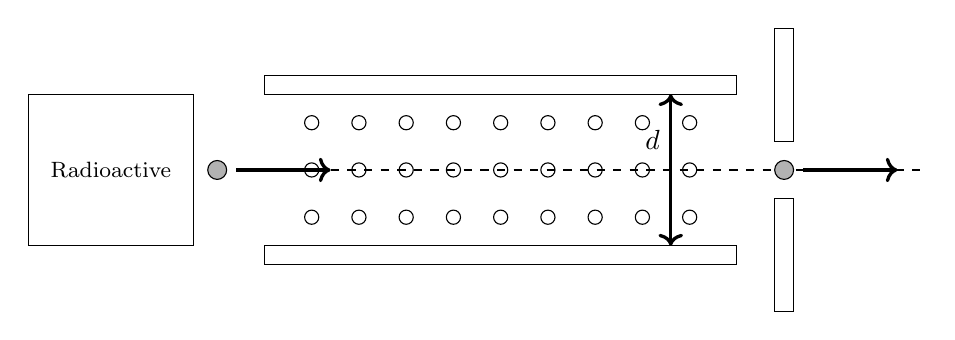
\begin{tikzpicture}[scale=1.2]
      \draw(0,0) rectangle(5,0.2);
      \draw(0,1.8) rectangle(5,2);
      \draw(-.75,0.2) rectangle(-2.5,1.8)
      node[midway]{\footnotesize Radioactive};
      \foreach \x in {.5,1,...,4.5}{
        \foreach \y in {.5,1,1.5} \draw(\x,\y) circle(0.075);
      }
      \draw[dashed](0,1)--(7,1);
      \draw[very thick,<->](4.3,.2)--(4.3,1.8) node[pos=.7,left]{$d$};
      \foreach \xx in {-.5,5.5}{
        \draw[fill=gray!60](\xx,1) circle (0.1);
        \draw[very thick,->](\xx+.2,1)--(\xx+1.2,1) node[midway,above]{$\varv$};
      }
      \draw(5.4,1.3) rectangle(5.6,2.5);
      \draw(5.4,0.7) rectangle(5.6,-.5);
    \end{tikzpicture}
  }

  \question A lead box containing radioactive materials that emit both
  electrons and positrons is placed near an apparatus consisting of an
  evacuated capacitor that is filled with a magnetic field, as shown in the
  figure above. Electrons that enter along the center line of the capacitor
  plates travel straight through (undeflected) with a velocity of
  $\varv=\SI{1.0e7}{\metre\per\second}$ and out the hole in the center of the
  apparatus on the right. The capacitor plates are separated by a distance of
  $d=\SI{.020}\metre$; each plate has an area of $A=\SI{1.0e-4}{\metre\squared}$
  and a potential difference of $\Delta V$. A uniform magnetic field of
  $B=\SI{0.030}\tesla$ is directed out of the page between the plates, as shown
  in the figure.
  \begin{parts}
    \part Explain why it is acceptable to neglect the effects of gravity on the
    electrons passing through the apparatus.
    \part
    \begin{subparts}
      \subpart Explain why the electrons pass through the capacitor plates
      undeflected. Support your argument with an algebraic equation
      and an appropriately drawn force diagram.

      \subpart Use your equation to calculate the potential difference
      ($\Delta V$) between the capacitor plates.

      \subpart Which capacitor plate has the highest potential? Justify your 
      reasoning making reference to the electric field.

      \subpart Calculate the magnitude of the energy that is stored in the
      capacitor.
    \end{subparts}

    \part A positron enters the apparatus along the same path as the electrons
    from part (b).
    \begin{subparts}
      \subpart Explain why the positron, traveling at the same speed as the
      electrons, will also travel straight through the device undeflected.
      Support your argument with an equation.
      
      \subpart A second positron enters the apparatus at a speed of $2\varv$.
      Sketch the path of the positron through the capacitor plates on the
      figure.
    \end{subparts}

    \part An electron exits the apparatus at a velocity of
    $\varv=\SI{1.0e7}{\metre\per\second}$ parallel to a long wire of a circuit,
    as shown in the figure. The distance between the electron and the wire is
    \SI1{\milli\metre}.
    \begin{center}
      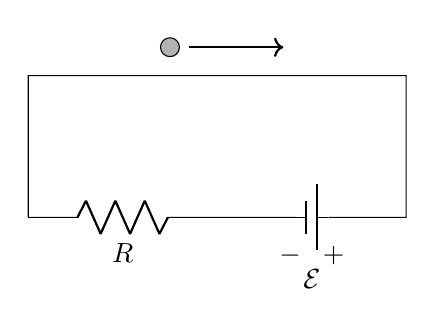
\begin{tikzpicture}[american voltages,scale=1.2]
        \draw(0,-.5)--(0,1)--(4,1)--(4,-.5) to[battery1=$\mathcal E$] (2,-.5)
        to[R=$R$] (0,-.5);
        \draw[fill=gray!60](1.5,1.3) circle (0.1);
        \draw[thick,->](1.7,1.3)--(2.7,1.3) node[midway,above]{$\varv$};
      \end{tikzpicture}
    \end{center}
    \begin{subparts}
      \subpart Calculate the potential difference-to-resistance ratio of the
      circuit such that the electron will experience a force $F$ of
      \SI{1.3e-16}\newton.
      
      \subpart Draw a force vector on the figure to show the direction of the
      force on the electron.
    \end{subparts}
  \end{parts}
  \newpage
  
%  %TAKEN FROM 2002 AP PHYSICS C FREE-RESPONSE QUESTION E&M 3
%  \uplevel{
%    \cpic{.65}{flux-through-loop}
%  
%  \question A circular wire loop with radius \SI{.10}{\metre} and resistance
%  \SI{50}{\ohm} is suspended horizontally in a magnetic field of magnitude $B$
%  directed upward at an angle of \ang{60} with the vertical, as shown above.
%  The magnitude of the field in teslas is given as a function of time $t$ in
%  seconds by the equation $B=4(1-0.2t)$.
%  \begin{parts}
%    \part Determine the magnetic flux $\Phi_m$ through the loop as a function of
%    time.
%    
%    \part Graph the magnetic flux $\Phi_m$ as a function of time on the axes
%    below.
%    \begin{center}
%      \begin{tikzpicture}[yscale=1.2]
%        \draw[very thick,->](-.1,0)--(11,0) node[pos=0,left]{0}
%        node[right]{$t$ (s)};
%        \draw[very thick,->](0,-2.3)--(0,3)
%        node[above]{$\Phi_m$ (\si{\tesla.\metre\squared})};
%        \foreach\x in {1,...,10}{
%          \draw[thick,dashed](\x,-2.3)--(\x,2.7);
%          \node[fill=white,below] at (\x,-.03) {$\x$};
%        }
%        \foreach\y in {-0.1,-0.05,0.05,0.1}
%        \draw[thick,dashed](0,\y*20)--(10.7,\y*20) node[pos=0,left]{$\y$};
%        \foreach\y in {-2,-1.8,...,2.2} \draw(-.1,\y)--(.1,\y);
%      \end{tikzpicture}
%    \end{center}
%    
%    \part Determine the magnitude of the induced emf in the loop.
%
%    \part
%    \begin{subparts}
%      \subpart Determine the magnitude of the induced current in the loop.
%      \subpart Show the direction of the induced current on the following
%      diagram.
%    \end{subparts}
%    \cpic{.65}{flux-through-loop}
%  \end{parts}
%  \newpage
%
%  % TAKEN FROM 2004 AP PHYSICS C EXAM FREE-RESPONSE QUESTION E&M 3. THERE ARE
%  % A LOT OF PROBLEMS THAT ARE VERY SIMILAR TO THIS ONE.
%  \uplevel{
%    \centering
%    \begin{tikzpicture}
%      \draw[thick](0,0) rectangle(4,3);
%      \draw[|<->|](0,3.3)--(4,3.3) node[midway,fill=white]{$4\ell$};
%      \draw[|<->|](-.4,0)--(-.4,3) node[midway,fill=white]{$3\ell$};
%      \draw[|<->|](-.4,0)--(-.4,-1) node[midway,fill=white]{$\ell$};
%      \draw[thick,->](-2,-1)--(2,-1) node[below]{$I$};
%      \draw[thick](1.9,-1)--(6,-1);
%    \end{tikzpicture}
%  }
%  \question A rectangular loop of dimensions $3\ell$ and $4\ell$ lies in the
%  plane of the page as shown above. A long straight wire also in the plane of
%  the page carries a current $I$.
%  \begin{parts}
%    \part Calculate the magnetic flux through the rectangular loop in terms of
%    $I$, $\ell$, and fundamental constants.
%    
%    \uplevel{
%      Starting at time $t=0$, the current in the long straight wire is given as
%      a function of time $t$ by $I(t)=I_0e^{-kt}$, where $I_0$ and $k$ are
%      constants.
%    }
%
%    \part The current induced in the loop is in which direction? Justify your
%    answer.
%
%    \vspace{.15in}
%    \underline{\hspace{.5in}} Clockwise \hspace{1in}
%    \underline{\hspace{.5in}} Counterclockwise
%
%    \uplevel{
%      The loop has a resistance $R$. Calculate each of the following in terms
%      of $R$, $I_0$, $k$, $\ell$, and fundamental constants.
%    }
%    \part The current in the loop as a function of time $t$
%    
%    \part The total energy dissipated in the loop from $t=0$ to $t=\infty$
%  \end{parts}
%  \newpage
%
%  \uplevel{
%    \centering
%    \begin{tikzpicture}[scale=.5]
%      \draw[very thick,->](0,1)  arc(90:270:7 and 1) node[below]{$I$};
%      \draw[very thick](-.1,-1) arc(-91:91:7 and 1);
%      \fill(0,0) circle(.08);
%      \draw[thick,<->](-7,0)--(0,0) node[midway,fill=white]{$R$};
%      \draw[thick,<->](0,3.5)--(0,0) node[midway,fill=white]{$R/2$};
%      \fill(0,3.5) circle(.1) node[right]{$P$};
%    \end{tikzpicture}
%    
%    Figure 1
%  }
%  \question The circular loop of wire in Figure 1 above has a radius of $R$ and
%  carries a current $I$. Point $P$ is a distance of $R_2$ above the center of
%  the loop. Express algebraic answers to parts (a) and (b) in terms of $R$,
%  $I$, and fundamental constants.
%  \begin{parts}
%    \part
%    \begin{subparts}
%      \subpart State the direction of the magnetic field $B_1$ at point $P$ due
%      to the current in the loop.
%      
%      \subpart Calculate the magnitude of the magnetic field $B_1$ at point $P$.
%    \end{subparts}
%
%    \uplevel{
%      \begin{center}
%        \begin{minipage}{.45\textwidth}
%          \centering
%          \begin{tikzpicture}[scale=.5]
%            \draw[very thick,->](0,1)  arc(90:270:7 and 1) node[below]{$I$};
%            \draw[very thick](-.1,-1) arc(-91:91:7 and 1);
%            \fill(0,0) circle(.08);
%            \draw[thick,<->](-7,0)--(0,0) node[midway,fill=white]{$R$};
%            \draw[thick,<->](0,3.5)--(0,0) node[midway,fill=white]{$R/2$};
%            \fill(0,3.5) circle(.1) node[right]{$P$};
%            
%            \draw[very thick,->](0,8)  arc(90:270:7 and 1) node[below]{$I$};
%            \draw[very thick](-.1,6) arc(-91:91:7 and 1);
%            \fill(0,7) circle(.08);
%            
%            \draw[thick,<->](-7,0)--(-7,7) node[midway,fill=white]{$R$};
%          \end{tikzpicture}
%        
%          Figure 2
%        \end{minipage}
%        \begin{minipage}{.45\textwidth}
%          \centering
%          \begin{tikzpicture}[scale=.5]
%            \draw[very thick,->](0,1)  arc(90:270:7 and 1) node[below]{$I$};
%            \draw[very thick](-.1,-1) arc(-91:91:7 and 1);
%            \fill(0,0) circle(.08);
%            \draw[thick,<->](-7,0)--(0,0) node[midway,fill=white]{$R$};
%            \fill(0,3.5) circle(.1) node[right]{$P$};
%            
%            \draw[very thick,->](0,8)  arc(90:270:7 and 1) node[below]{$I$};
%            \draw[very thick](-.1,6) arc(-91:91:7 and 1);
%            \fill(0,7) circle(.08);
%            
%            \draw[dashed](-1.7,3.5)--(2,3.5) node[right]{Axis};
%            \draw[very thick](-1.5,2.8)--(1.5,2.8) node[midway,below]{$s$}
%            --(1,4.2)--(-1,4.2)--cycle;
%          \end{tikzpicture}
%
%          Figure 3
%        \end{minipage}
%      \end{center}
%      
%      \vspace{.2in}A second identical loop also carrying a current $I$ is added
%      at a distance of $R$ above the first loop, as shown in Figure 2 above.
%    }
%
%    \part Determine the magnitude of the net magnetic field $B$ net at point
%    $P$.
%
%    \uplevel{
%      A small square loop of wire in which each side has a length $s$ is now
%      placed at point $P$ with its plane parallel to the plane of each loop, as
%      shown in Figure 3 above. For parts (c) and (d), assume that the magnetic
%      field between the two circular loops is uniform in the region of the
%      square loop and has magnitude $B_\text{net}$.
%    }
%    
%    \part In terms of $B_\text{net}$ and $s$, determine the magnetic flux
%    through the square loop.
%
%    \part The square loop is now rotated about an axis in its plane at an
%    angular speed $\omega$. In terms of $B_\text{net}$ , $s$, and $\omega$,
%    calculate the induced emf in the loop as a function of time $t$, assuming
%    that the loop is horizontal at $t=0$.
%  \end{parts}
%  \newpage
  
  \question A section of a long conducting cylinder with inner radius $a$ and
  outer radius $b$ carries a current $I_0$ that has a uniform current density,
  as shown in the figure above.
  \begin{parts}
    \part Using Amp\`{e}re's law, derive an expression for the magnitude of
    the magnetic field in the following regions as a function of the distance
    $r$ from the central axis.
    \begin{subparts}
      \subpart $r<a$
      \subpart $a<r<b$
      \subpart $r=2b$
    \end{subparts}
    
    \part On the cross-sectional view in the diagram above, indicate the
    direction of the field at point $P$, which is at a distance $r=2b$ from the
    axis of the cylinder.

    \part An electron is at rest at point $P$. Describe any electromagnetic
    forces acting on the electron. Justify your answer.

    \uplevel{
      Now consider a long, solid conducting cylinder of radius $b$ carrying a
      current $I_0$. The magnitude of the magnetic field inside this cylinder
      as a function of $r$ is given by $B=\mu_0I_0r/2\pi b^2$. An experiment is
      conducted using a particular solid cylinder of radius \SI{.010}{\metre}
      carrying a current of \SI{25}{\ampere}. The magnetic field inside the
      cylinder is measured as a function of $r$, and the data is tabulated
      below.

      \vspace{.2in}
      \begin{center}
        \begin{tabular}{|l|l|l|l|l|l|}
          \hline
          Distance $r$ (m)    & 0.002 & 0.004 & 0.006 & 0.008 & 0.010\\ \hline
          Magnetic Field $B$ (T) & \num{1.2e-4} & \num{2.7e-4} & \num{3.6e-4}
          & \num{4.7e-4} & \num{6.4e-4} \\
          \hline
        \end{tabular}
      \end{center}
    }
    
    \part
    \begin{subparts}
      \subpart On the graph below, plot the data points for the magnetic field
      $B$ as a function of the distance $r$, and label the scale on both axes.
      Draw a straight line that best represents the data.
      \begin{center}
        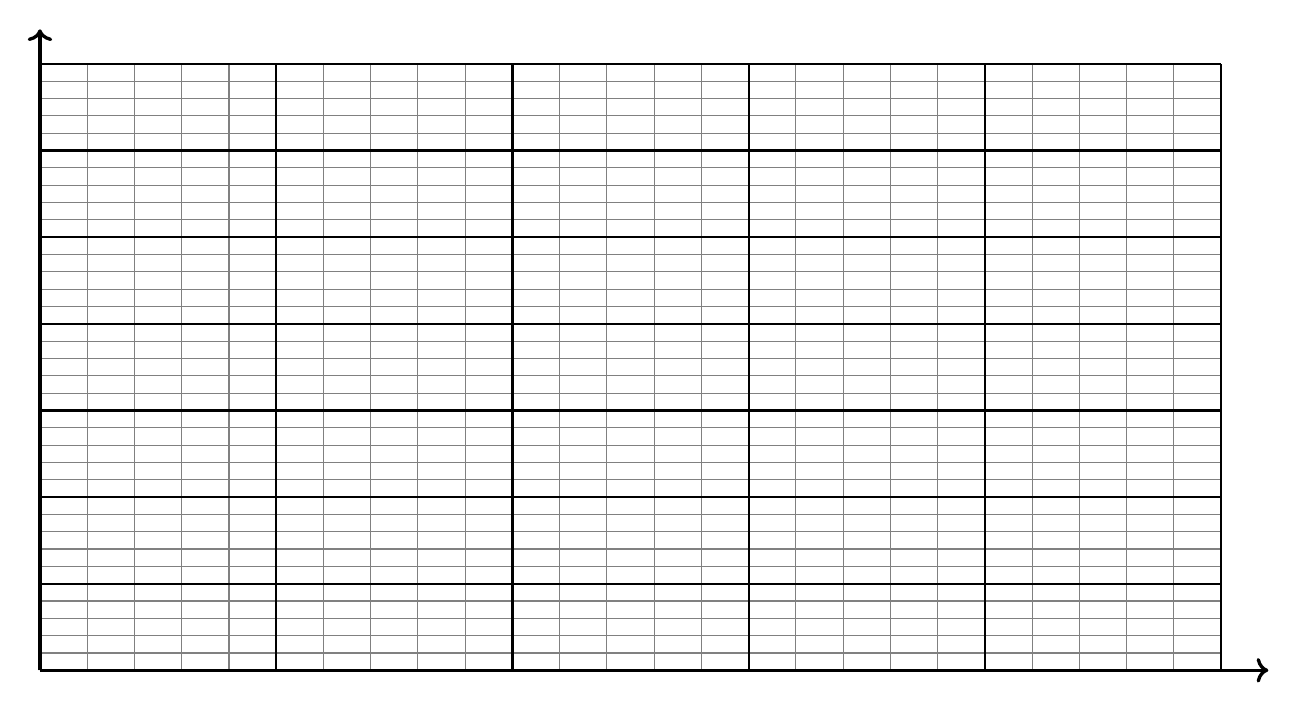
\begin{tikzpicture}[xscale=.6,yscale=.22]
          \draw[gray](0,0) grid(25,35);
          \draw[very thick,->](0,0)--(26,0);
          \draw[very thick,->](0,0)--(0,37);
          \draw[thick,step=5](0,0) grid(25,35);
        \end{tikzpicture}
      \end{center}
      \subpart Use the slope of your line to estimate a value of the
      permeability $\mu_0$.
    \end{subparts}
  \end{parts}
  \newpage

%  \uplevel{
%    \cpic{.5}{inout}
%  }
%  \question The rectangular loop of wire shown on the left in the figure above
%  has mass $M$, length $L$, width $L/4$, and resistance $R$. It is initially
%  moving to the right at constant speed $\varv_0$ , with no net force acting on
%  it. At time $t=0$ the loop enters a region of length $2L$ that contains a
%  uniform magnetic field of magnitude $B$ directed into the page. The loop
%  emerges from the field at time $t_f$ with final speed $\varv_f$. Express all
%  algebraic answers to the following in terms of $M$, $L$, $R$, $B$, $\varv_0$,
%  and fundamental constants, as appropriate.
%  \begin{parts}
%    \part Let $x$ represent the position of the right end of the loop. Place a
%    check mark in the appropriate box in each column in the table below to
%    indicate whether the speed of the loop increases, decreases, or stays the
%    same as the loop moves to the right.
%
%
%    \part Derive an expression for the magnitude of the current induced in the
%    loop as its right edge enters the field.
%
%    \part What is the direction of the induced current determined in part (b) ?
%    Justify your answer.
%
%    \vspace{.15in}
%    \underline{\hspace{.5in}} Clockwise\hspace{.6in}
%    \underline{\hspace{.5in}} Counterclockwise
%    
%    \part Write, but do not solve, a differential equation for the speed
%    $\varv$ as a function of time as the loop enters the field.
%    
%    \part What is the direction of the acceleration of the loop just before
%    its left edge leaves the field? Justify your answer.
%
%    \vspace{.15in}
%    \underline{\hspace{.5in}} Left\hspace{1in}
%    \underline{\hspace{.5in}} Right\hspace{1in}
%    \underline{\hspace{.5in}} Up\hspace{1in}
%    \underline{\hspace{.5in}} Down
%  \end{parts}
%  \newpage
%
%  \uplevel{
%    \centering
%    \begin{tikzpicture}[scale=1.2]
%      \foreach \x in {0,...,3}{
%        \foreach \y in {0,...,4}
%        \node at (\x,\y){\textcolor{black!80}{$\bm\times$}};
%      }
%      \draw[thick,fill=gray!70](.5,2.25) rectangle(2.5,2.5)
%      node[above,midway]{$M$, $L$};
%      \draw[thick](.5,.5)--(.5,3.7) node[pos=0,left]{$B$}
%      to[R,l=$R$](2.5,3.7)--(2.5,.5);
%      \fill (1.5,1.5) circle(.06) node[right]{$D$};
%      \fill (1.5,3.2) circle(.06) node[right]{$C$};
%      \draw[very thick,->](4.5,3)--(4.5,2) node[below]{Vertically down};
%    \end{tikzpicture}
%  }
%  \question A conducting bar of mass $M$, length $L$, and negligible resistance
%  is connected to two long vertical conducting rails of negligible resistance.
%  The two rails are connected by a resistor of resistance $R$ at the top. The
%  entire apparatus is located in a magnetic field of magnitude $B$ directed
%  into the page, as shown in the figure above. The bar is released from rest
%  and slides without friction down the rails.
%  \begin{parts}
%    \part What is the direction of the current in the resistor?
%
%    \vspace{.15in}
%    \underline{\hspace{.5in}} Left\hspace{1in}
%    \underline{\hspace{.5in}} Right
%
%    \part
%    \begin{subparts}
%      \subpart Is the magnitude of the net magnetic field above the bar at
%      point $C$ greater than, less than, or equal to the magnitude of the net
%      magnetic field before the bar is released? Justify your answer.
%
%      \vspace{.15in}
%      \underline{\hspace{.5in}}Greater than\hspace{1in}
%      \underline{\hspace{.5in}}Less than\hspace{1in}
%      \underline{\hspace{.5in}}Equal to
%      \vspace{.1in}
%      
%      \subpart While the bar is above point $D$, is the magnitude of the net
%      magnetic field at point $D$ greater than, less than, or equal to the
%      magnitude of the net magnetic field before the bar is released?
%      Justify your answer.
%
%      \vspace{.15in}
%      \underline{\hspace{.5in}}Greater than\hspace{1in}
%      \underline{\hspace{.5in}}Less than\hspace{1in}
%      \underline{\hspace{.5in}}Equal to
%      \vspace{.1in}
%    \end{subparts}
%    
%    \uplevel{
%      Express your answers to parts (c) and (d) in terms of $M$, $L$, $R$, $B$,
%      and physical constants, as appropriate.
%    }
%
%    \part Write, but do NOT solve, a differential equation that could be used
%    to determine the velocity of the falling bar as a function of time $t$.
%    
%    \part Determine an expression for the terminal velocity $v_T$ of the bar.
%
%    \uplevel{
%      Express your answers to parts (e) and (f) in terms of $v_T$, $M$, $L$,
%      $R$, $B$, and physical constants, as appropriate.
%    }
%    
%    \part Derive an expression for the power dissipated in the resistor when
%    the bar is falling at terminal velocity.
%
%    \part Using your differential equation from part (c), derive an expression
%    for the speed of the falling bar $v_t$ as a function of time $t$.
%  \end{parts}

  
  % TAKEN FROM 2004 AP PHYSICS C EXAM FREE-RESPONSE QUESTION E&M 2.
  % THIS QUESTION IS BETTER SUITED FOR THE ELECTRIC CIRCUIT SECTION, BUT IS
  % HERE FOR SOME REASON. I MIGHT MOVE IT TO HW 16 LATER.
  
%  \cpic{.85}{RC2004}
%  \question In the circuit shown above left, the switch $S$ is initially in the
%  open position and the capacitor $C$ is initially uncharged. A voltage probe
%  and a computer (not shown) are used to measure the potential difference
%  across the capacitor as a function of time after the switch is closed. The
%  graph produced by the computer is shown above right. The battery has an emf
%  of \SI{20}{\volt} and negligible internal resistance. Resistor $R_1$ has a
%  resistance of \SI{15}{\kilo\ohm} and the capacitor $C$ has a capacitance of
%  \SI{20}{\micro\farad}.
%  \begin{parts}
%    \part Determine the voltage across resistor $R_2$ immediately after the
%    switch is closed.
%    
%    \part Determine the voltage across resistor $R_2$ a long time after the
%    switch is closed.
%    
%    \part Calculate the value of the resistor $R_2$.
%    
%    \part Calculate the energy stored in the capacitor a long time after the
%    switch is closed.
%    
%    \part On the axes below, graph the current in $R_2$ as a function of time
%    from 0 to \SI{15}{\second}. Label the vertical axis with appropriate
%    values.
%    \begin{center}
%      \begin{tikzpicture}[xscale=.6,yscale=.35]
%        \draw[dashed](0,0) grid(15,20);
%        \draw[step=5,very thick](0,0) grid(15,20);
%        \foreach \x in {0,5,...,15} \node[below] at (\x,0) {$\x$};
%        \node[below] at (7.5,-1.5) {Time (s)};
%        \node[left] at (0,10) {Current in $R_2$};
%      \end{tikzpicture}
%    \end{center}
%    \uplevel{
%      Resistor $R_2$ is removed and replaced with another resistor of lesser
%      resistance. Switch $S$ remains closed for a long time.
%    }
%
%    \part Indicate below whether the energy stored in the capacitor is greater
%    than, less than, or the same as it was with resistor $R_2$ in the circuit.
%    Explain your reasoning.
%    
%    \vspace{.1in}
%    \underline{\hspace{.2in}} Greater than\hspace{.3in}
%    \underline{\hspace{.2in}} Less than\hspace{.3in}
%    \underline{\hspace{.2in}} The same as
%  \end{parts}
%  \newpage

%\item Two positive charges $+q$ are on the $y$ axis at $y=+a$ and $y=-a$.
%  \begin{enumerate}
%  \item Show that the electric field on the $x$ axis is along the $x$ axis with
%    $E_x=2kqx(x^2+a^2)^{-3/2}$.
%  \item Show that near the origin, when $x\ll a$, $E_x\approx 2kqx/a^3$.
%  \item Show that for $x\gg a$, $E_x\approx 2kq/x^2$.
%  \item Explain why you should expect the result in (c) even before calculating
%    it.
%  \end{enumerate}
%  A bead of mass $m$ with a negative charge $-q$ slides along a thread that
%  runs along the $x$ axis.
%  \begin{enumerate}[resume]
%  \item Show that for small displacements $x\ll a$, the bead experiences a
%    restoring force that is proportional to $x$ and therefore undergoes
%    simple harmonic motion.
%  \item Find the period of the motion.
%  \end{enumerate}
%  %\vspace{\stretch{4}}
%  \newpage
%  
%\item Using Gauss's law, find
%  \begin{enumerate}
%  \item the electric field strength inside and outside of a uniformly charged
%    hollow sphere of radius $R$ and surface charge density $\sigma$ (charge
%    per unit area).
%  \item the electric field inside and outside an infinitely long cyclindrical
%    shell of charge of radius $R$ with charge discibution $\sigma$ (charge
%    per unit area).
%  \item the electric field strength inside and outside a infinitely long solid
%    cylinder of radius $R$ carrying a linear uniform charge density $\rho$
%    (charge per unit volume).
%  \end{enumerate}
%  Hint: In all cases, think about where to put the Gaussian surface. Take
%  advantage of symmetry.
%  %\vspace{\stretch{1}}
%  \newpage

%\item A parallel-plate capacitor has a capacitance $C_0$ and plate separation
%  of $d$. To dielectric slabs of constants $\kappa_1$ and $\kappa_2$, each of
%  thickness $d/2$ and having the same area as the plates, are inserted between
%  the plates as shown in the figure below. When the free charge on the plates
%  are $Q$,
%  \begin{enumerate}
%  \item find the electric field in each of the dielectric
%  \item find the potential difference between the plates
%  \item show that the new capacitance is given by:
%    $C=\dfrac{\kappa_1\kappa_2}{\kappa_1+\kappa_2}C_0$
%  \end{enumerate}
%  \cpic{.2}{stacked}
\end{questions}
\end{document}
